% Chapter Template

\chapter{Ensayos y Resultados} % Main chapter title

\label{Chapter4} % Change X to a consecutive number; for referencing this chapter elsewhere, use \ref{ChapterX}

Este capítulo expone las características del dispositivo desarrollado en contraste con los requerimientos de diseño y los casos de uso.
%----------------------------------------------------------------------------------------
%	SECTION 1
%----------------------------------------------------------------------------------------

\section{Análisis de casos de uso y cumplimiento de los requerimientos}
\label{sec:pruebasHW}

\textbf{Caso de uso CU001: Autonomía}

El primer caso de uso analizado está relacionado a la autonomía del equipo. Se midió el consumo del equipo en diferentes situaciones en la que no está conectado por USB y se muestra en la Tabla \ref{tab:autonomia}.

\begin{table}[h]
\caption{Autonomía del Equipo}
\label{tab:autonomia}
\begin{tabular}{@{}llll@{}}
\toprule
\textbf{Fase}                       & \textbf{\begin{tabular}[c]{@{}l@{}}Consumo\\ promedio\end{tabular}} & \textbf{\begin{tabular}[c]{@{}l@{}}Duración \\ estimada\end{tabular}} & \textbf{Descripción}                                                                                                \\ \midrule
Espero conexión BT                  & I$_0$ = 78mA                                                         & t$_0$ = 30 min                                                         & \begin{tabular}[c]{@{}l@{}}Instalo el equipo y \\ conecto sensores\end{tabular}                                     \\
Configuración previa a experiencia  & I$_1$ = 65mA                                                         & t$_1$ = 30 min                                                          & \begin{tabular}[c]{@{}l@{}}Envío señal de prueba, \\ configuro parámetros\end{tabular}                              \\
Equipo conectado BT inactivo        & I$_2$ = 62 mA                                                        & t$_2$ = 10 min                                                          & \begin{tabular}[c]{@{}l@{}}Modificación de la \\ instalación del equipo \\ (sujeción, conectores, etc)\end{tabular} \\
Equipo adquiriendo sin enviar señal & I$_3$ = 45 mA                                                        & t$_3$ = 24 hs                                                           & Experiencia                                                                                                         \\
Acceso a ver señal                  & I$_4$ = 75 mA                                                       & t$_4$ = 20 min                                                           & \begin{tabular}[c]{@{}l@{}}Accedo eventualmente a \\ ver la señal que se está\\ adquiriendo\end{tabular}            \\ \bottomrule
\end{tabular}
\end{table}

Se calculó el consumo medio teórico realizando el promedio ponderado de los consumos en las situaciones anteriores. Puede verse en la formula \ref{eqn:consumoMedio}

\begin{equation} \label{eqn:consumoMedio}
consumoMedio = I_{0}*t_{0}+I_{1}*t_{1}+I_{2}*t_{2}+I_{3}*t_{3}+I_{4}*t_{4} = 1186.3 mAh
\end{equation}



Asimismo, la corriente mediala podemos calcular dividiendo por el tiempo total, como en la fórmula \ref{eqn:corrienteMedia}. Esto nos permite estimar la eficiencia del regulador para esa tensión.

\begin{equation} \label{eqn:corrienteMedia}
I_{med} = \frac{I_{0}*t_{0}+I_{1}*t_{1}+I_{2}*t_{2}+I_{3}*t_{3}+I_{4}*t_{4}}{t_{0}+t_{1}+t_{2}+t_{3}+t_{4}}= 46.54mA
\end{equation}

De acuerdo a la hoja de datos del regulador TPS63001 \citep{texas2006}, esta corriente media nos da una eficiencia de alrededor de 90\%, aunque este valor también depende de la tensión de la batería.
Se colocó en el equipo una pila en serie modelo TR18650 de 3.7V y una autonomía de 2400mAh, como muestra la figura \ref{fig:bateria}. El cálculo se realizó suponiendo una descarga lineal de la misma, desde su tensión inicial hasta la mínima tensión admisible para el regulador, que es de 1.8V\citep{texas2006} (este valor fue comprobado experimentalmente). El porcentaje de descarga de la pila antes de que el regulador deje de funcionar se calcula en la fórmula \ref{eqn:porcentajeDescarga}.

\begin{equation} \label{eqn:porcentajeDescarga}
porcentajeDescarga = \frac{V_{ini} - V_{fin}}{V_{ini}} * 100\% = \frac{3.7V- 1.8V}{3.7V} * 100\% = 51.35\%
\end{equation}

\begin{figure}[!htbp]
	\centering	
	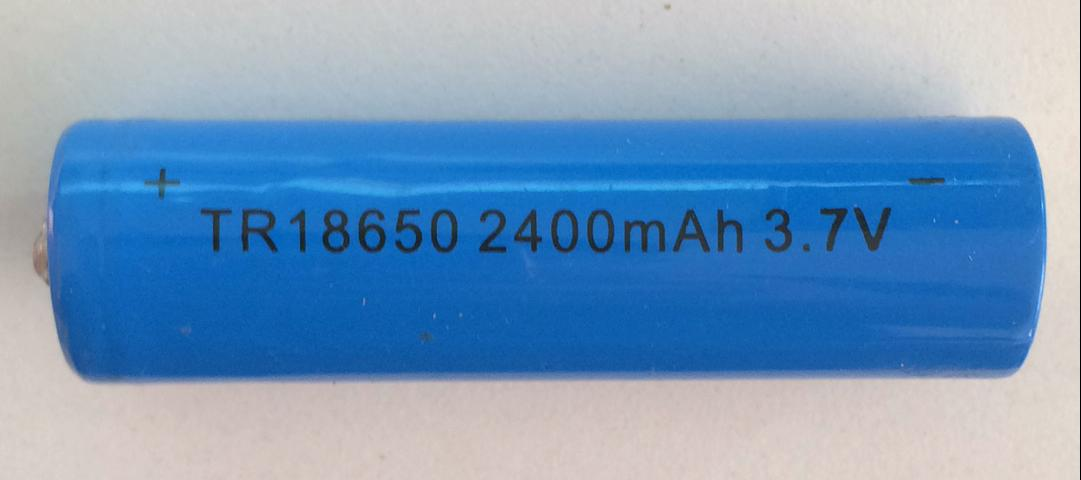
\includegraphics[width=0.9\textwidth]{./Figures/bateria.jpeg}			
	\caption{Batería TR18650 utilizada en el equipo}
	\label{fig:bateria}
\end{figure}

Teniendo en cuenta la eficiencia del 90\% y el porcentaje de descarga máxima de 51.35\%, la autonomía aprovechable de la batería será aproximadamente de 1109mAh, según lo calculado en la fórmula \ref{eqn:autonomiaReal}.
Este valor está cerca del consumo teórico calculado. 

\begin{equation} \label{eqn:autonomiaReal}
\begin{split}
autonomiaReal = autonomiaReal*eficiencia*porcentajeDescarga = \\ 2400mAh * 90\% * 51.35\% = 1109 mAh
\end{split}
\end{equation}

Se realizaron varias experiencias para verificar la autonomía del equipo y se obtuvieron en todas resultados similares. La duración de la batería fue de aproximadamente 22 horas. Puede verse la curva de descarga de una de las experiencias en la figura \ref{fig:descargaBateria}. En esta figura se decimaron las muestras obtenidas y se visualiza una medición cada media hora. El divisor resistivo de entrada del ADC conectado a la batería es de 330kOhm y 820kOhm, lo que da una relación de 0.287. Este valor se usó para convertir las muestras entregadas por el ADC a Volts.

\begin{figure} [!htpb]
    \centering
    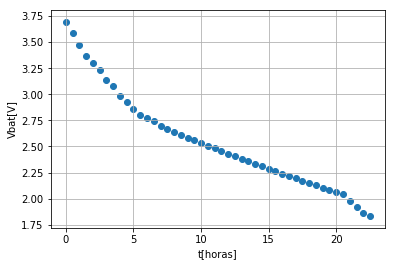
\includegraphics[width=\textwidth]{./Figures/descargaBateria.png}
    \caption{Descarga de la bateria durante experiencia}
    \label{fig:descargaBateria}
\end{figure}

Los requerimientos asociados a este caso de uso no son cubiertos completamente. Sin embargo, se puede solucionar colocando una pila de mayor autonomía como puede ser la indicada en el siguiente link : https://uk.rs-online.com/web/p/lithium-rechargeable-batteries/7760863/, que no fue adquirida por una cuestión de presupuesto.


\textbf{Caso de uso CU002: Configuración}

Para comprobar este caso de uso se inició con el equipo reiniciado por hardware. Se utilizó una tablet con Android y la aplicación Blueterm instalada. A través de la aplicación se enviaron los comandos para ingresar al modo configuración, y luego se modificaron cada uno de los parámetros, comprobando la escritura en las variables asociadas en RAM a través del debugger, y luego realizando diferentes mediciones para diferentes configuraciones. Estas mediciones fueron realizadas con señales provistas por un generador de señales UTG4082A excitando la entrada del amplificador operacional. En la figura \ref{fig:confPGA} puede visualizarse la misma señal generada adquirida con dos ganancias de PGA diferentes (1 y 2). El setup para la experiencia puede visualizarse en la figura \ref{fig:confPGAexp}.

\begin{figure} [!htpb]
    \centering
    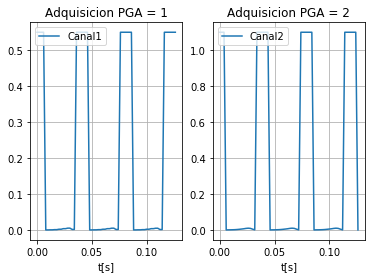
\includegraphics[width=\textwidth]{./Figures/confPGA.png}
    \caption{Señales adquiridas con PGA = 1 y PGA = 2}
    \label{fig:confPGA}
\end{figure}

\begin{figure} [!htpb]
    \centering
    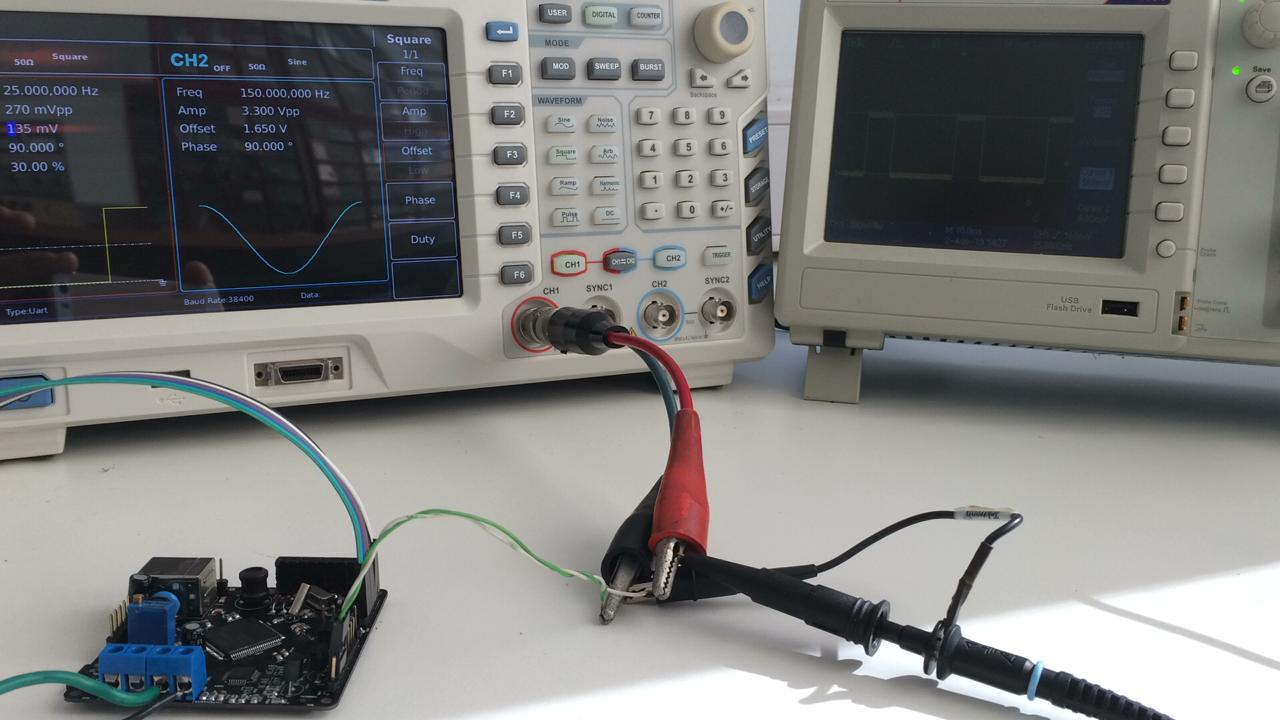
\includegraphics[width=\textwidth]{Figures/confPGAexp.jpeg}
    \caption{Señales adquiridas con PGA = 1 y PGA = 2}
    \label{fig:confPGAexp}
\end{figure}

Se realizó igualmente la configuración de habilitación de un solo canal (canal 1 y canal 2 por separado), la configuración de fecha y hora, y el muestreo a frecuencias de 500SPS, 250SPS y 125SPS.

También se realizó la rutina de calibración con uno de los sensores Königsberg, pero sin contar con un patrón de calibración de presión. Se comprobó unicamente la adquisición de valores diferentes de presión aplicando presión con el dedo y visualizando una medición mayor con su correspondiente incremento en el valor adquirido. El setup puede visualizarse en la figura \ref{fig:calibracion}. Resta comprobar la calibración con un patrón certificado de presión que sea adaptable a los sensores a utilizar. 

\begin{figure} [!htpb]
    \centering
    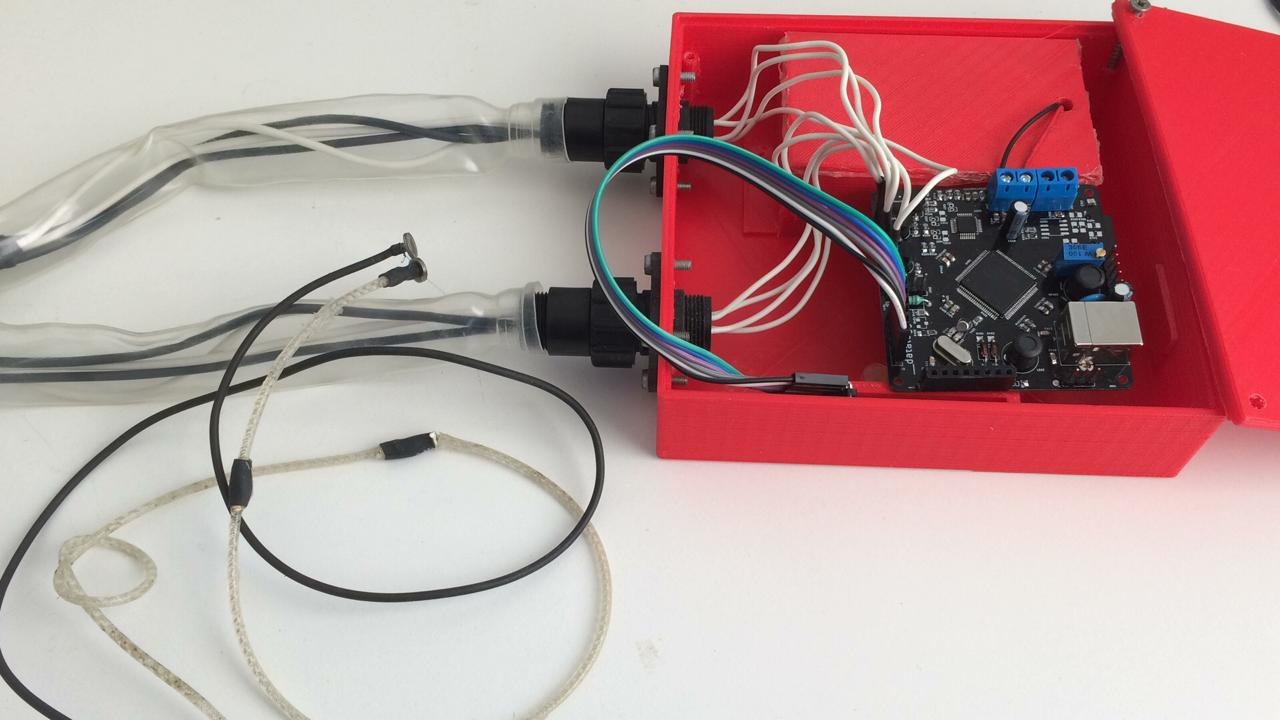
\includegraphics[width=\textwidth]{./Figures/calibracion.jpeg}
    \caption{Setup para calibración con sensores Königsberg}
    \label{fig:calibracion}
\end{figure}

\textbf{Caso de uso CU003: Experiencia}

Para este caso de uso se cargó la batería al 100\% y se operó el dispositivo desde una terminal con Android, utilizando la aplicación BlueTerm. Por tratarse de una prueba de funcionamiento, se utilizó el mismo setup que enel caso de la calibración, es decir, con los sensores a presión atmosférica. Se ingresó en el modo de ''adquirir+enviar'', con la configuración por default, es decir, con los dos canales habilitados, el PGA en ganancia unitaria, y una frecuencia de muestreo de 500SPS. 

Se comprobó el correcto envío de muestras truncadas a 16 bits y decimadas a 100Hz para no sobrecargar el módulo Bluetooth. Luego se pasó al modo ''adquirir+enviar+almacenar'' y finalmente al modo "adquirir+almacenar". Luego de 5 minutos, se interrumpió la experiencia para comprobar el correcto almacenamiento en la memoria micro SD. 
Se volvió a comenzar la experiencia de la misma manera pero esta vez no se interrumpió el almacenamiento y se continuó por 20 horas, finalmente se dio por terminada la experiencia. 

Esta secuencia se repitió pero intercalando ingresos a través de la aplicación Blueterm para consultar el envío de la señal online, de manera de comprobar que la visualización de la señal no altere el almacenamiento en la SD.
Se repitió el mismo procedimiento por cuarta vez, pero ahora utilizando el generador de señales para comprobar la adquisición de una señal conocida. 

La estrategia elegida para almacenar las señales fue generar archivos de hasta 50Mb para evitar problemas de copia o corrupción. Para obtener mejor rendimiento de velocidad al escribir y menor volumen de datos, toda la información se guardó en formato binario. En cada uno de los archivos se guardo información que contiene un número de identificación de la experiencia autonumerado, un índice que comienza en cero y que indica el número de archivo generado abierto durante la experiencia, la fecha en que se guardó el archivo, hora de inicio del archivo, valor de ganancia del PGA, cantidad de canales habilitados, y valor de la frecuencia de muestreo. En cada una de las muestras se guardaron 3 bytes por cada muestra por cada canal, ya que el ADC es de 24 bits y no tiene sentido guardar los 4 bytes de la variable donde se almacenan los valores. Además para cada valor se guarda 1 byte correspondientes a la batería, truncando la muestra de 12 bits del ADC interno. La información de hora y fecha solamente se guarda en el encabezado, y no en cada muestra.
Para poder visualizar estos archivos se creó un script de python que reune esta información y la escribe en un formato legible, además compagina todos los archivos generados por la experiencia, graficando las señales. Este script se realizó con fines de desarrollo, ya que la aplicación para visualización e interfaz con el equipo no alcanza los objetivos del presente trabajo. 

Resta por realizar las pruebas de aceptación en un caso real, con un animal instrumentado. Esta experiencia no pudo ser realizada dado los costos e impedimentos operativos, pero se planifica realizar en el corto plazo.

\textbf{Caso de uso CU004: Descarga de datos y carga de batería}

En todos las experiencias realizadas para el CU003 se descargaron los archivos via USB. Para el tamaño de archivos que se maneja no hubo ningún inconveniente y el equipo respondió correctamente.

La carga de batería se realiza una corriente constante de 100mA, por lo que una carga completa con la batería totalmente descargada toma 24 horas. En todos los casos, luego de cargar la batería, se comprobó que la tensión final de carga sea 3.7V utilizando un tester UNI-T PRO UT195DS. 